\chapter{Метрические пространства}


\section{Отображения}
Пусть $X,Y$ -- два множества, $R(x,y)$ -- отношение между $x \in X$, $y \in Y$. \textit{График} $\Gamma(R)$ отношения $R$ определяется следующим образом
\[
 X \times Y \supseteq \Gamma(R) : = \{(x,y) \, :\, (x,y) \in R\}.
\]

Пусть $X,Y$ -- два множества, $R(x,y)$ -- отношение между $x \in X$, $y \in Y$. Говорят, что $R$ \textit{функционально по $y$}, если для \textbf{каждого} $x\in X$ существует \textbf{один и только один} такой элемент $y\in Y$, что $R(x,y)$ истинно.

График $F$ такого отношения называется \textit{функциональным графиком} в $X \times Y$. Его можно также охарактеризовать следующим образом:  для каждого $x \in X$ существует один и только один такой элемент $y \in Y$, что $(x,y) \in R$; этот элемент называется \textit{значением} $F$ в $x$ и обозначается символом $F(x)$.

Функциональный график в $X \times Y$ называется также \textit{отображением $X$ в $Y$} или \textit{функцией, определённой в $X$ и принимающей значения в $Y.$}

Мы также будем записывать такое отображение в виде $F:X \to Y$, понимая под этим, что каждому $x \in X$ ставится в соответствие ровно один $y  = F(x)\in Y$. Множество $F(X) \subseteq Y$, определённое как $\{F(x), \, x \in X\}$, называется образом отображения $F$ и иногда будет обозначаться как $\mathrm{Im}(F).$ Далее, множество $F^{-1}(Y) \subseteq X$, определённое как
\[
 F^{-1}(Y):= \{x \in X\, :\, F(x) \in Y\},
\]
называется \textit{прообразом} отображения $F.$

\section{Пространство $\mathbb{R}^n$}

\begin{definition}
    
Множество, обозначаемое через $\mathbb{R}^n$, определятся следующим образом
\[
 \mathbb{R}^n: = \underbrace{\mathbb{R} \times \cdots \times  \mathbb{R}}_n.
\]

При этом, для любых $\alpha,\beta \in \mathbb{R}$, и $\mathbf{x}=(x_1,\ldots, x_n), \mathbf{y} = (y_1,\ldots, y_n) \in \mathbb{R}^n$;
\[
 \alpha \mathbf{x} + \beta \mathbf{y}: = (\alpha x_1 + \beta y_1, \ldots, \alpha x_n + \beta y_n). 
\]
\end{definition}


Таким образом, $\mathbb{R}^n$ -- это линейное пространство или векторное пространство над $\mathbb{R}$.

Когда мы будем говорить об $\mathbb{R}^n$ как о векторном пространстве, то каждый набор будем записывать как вектор, \ie в виде $\mathbf{x} = \begin{pmatrix} x_1 \\ \vdots \\ x_n \end{pmatrix} = (x_1,\ldots, x_n)^\top.$

Возьмём $\mathbf{x} = (x_1,\ldots, x_n)^\top \in \mathbb{R}^n$, тогда ясно, что 
\[
\begin{pmatrix}
    x_1 \\ \vdots \\x_n 
\end{pmatrix} = x_1 \begin{pmatrix}
    1 \\ \vdots \\ 0
\end{pmatrix} + \cdots + x_n \begin{pmatrix}
    0 \\ \vdots \\1
\end{pmatrix}
\]

Множество $\mathbb{e} = \{\mathbf{e}_1, \ldots, \mathbf{e}_n\}$, где $\mathbf{e}_1 = (1,0, \ldots, 0)^\top, \ldots, \mathbf{e}_n = (0,0,\ldots, 1)^\top$, называется \textit{базисом} пространства $\mathbb{R}^n.$

\subsection{Отображения в $\mathbb{R}^n$}

\textit{Линейное отображение} $f:\mathbb{R}^n \to \mathbb{R}^m$ -- это такое отображение, что $f(\alpha \m{x} +\beta \m{y]} ) = \alpha f(\m{x}) +\beta f(\m{y})$, где $\m{x,y} \in \mathbb{R}^n$, $\alpha, \beta \in \mathbb{R}.$ 

\begin{mydanger}{\bf{!}}
    Геометрически это означает, что образ прямой -- это опять прямая.
\end{mydanger}

В таком случае, линейное отображение $f:\mathbb{R}^n \to \mathbb{R}^m$ достаточно задать на базисных векторах и мы получаем что-то вроде

\[
 \begin{pmatrix}
     1 \\ \vdots \\ 0
 \end{pmatrix} \mapsto \begin{pmatrix}
     a_{11} \\ \vdots \\ a_{m1}
 \end{pmatrix}, \ldots, \begin{pmatrix}
     0 \\ \vdots \\ 1
 \end{pmatrix} \mapsto \begin{pmatrix}
     a_{1n} \\ \vdots \\ a_{mn}
 \end{pmatrix},
\]
что и кодируется матрицей 
$A = \begin{pmatrix}
    a_{11} & \ldots & a_{1n} \\
    \vdots & \ddots & \vdots \\
    a_{m1} & \ldots & a_{mn}
\end{pmatrix}$

\begin{figure}[h!]
    \centering
    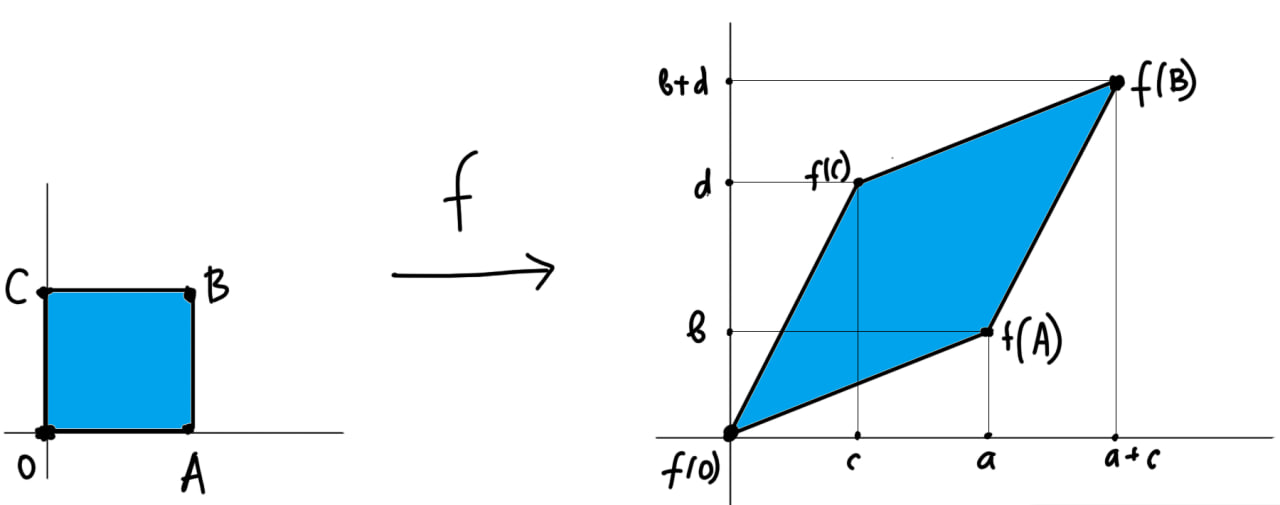
\includegraphics[scale = 0.5]{linear_map.jpg}
    \caption{Линейное отображение $f:\mathbb{R}^2 \to \mathbb{R}^2$, которое задаётся матрицей $A = \begin{pmatrix}
        a & c \\
        b & d
    \end{pmatrix}.$}
    \label{linear_map}
\end{figure}

Скажем также, что если у нас есть два линейных отображения $f:\mathbb{R}^n \to \mathbb{R}^k$, $g:\mathbb{R}^k \to \mathbb{R}^m$, закодированные матрицами $A$ и $B$ соответственно, то отображение $g \circ f: \mathbb{R}^n \to \mathbb{R}^k$ будет задаваться \sout{этим странным умножением матриц строка на столбец!!!} умножением матриц $BA$.

Но понятно, что одними только линейными всё не ограничивается. Ведь вовсе не обязательно, что образ прямой будет всегда прямая при любом её отображении.


\begin{figure}
    \centering
    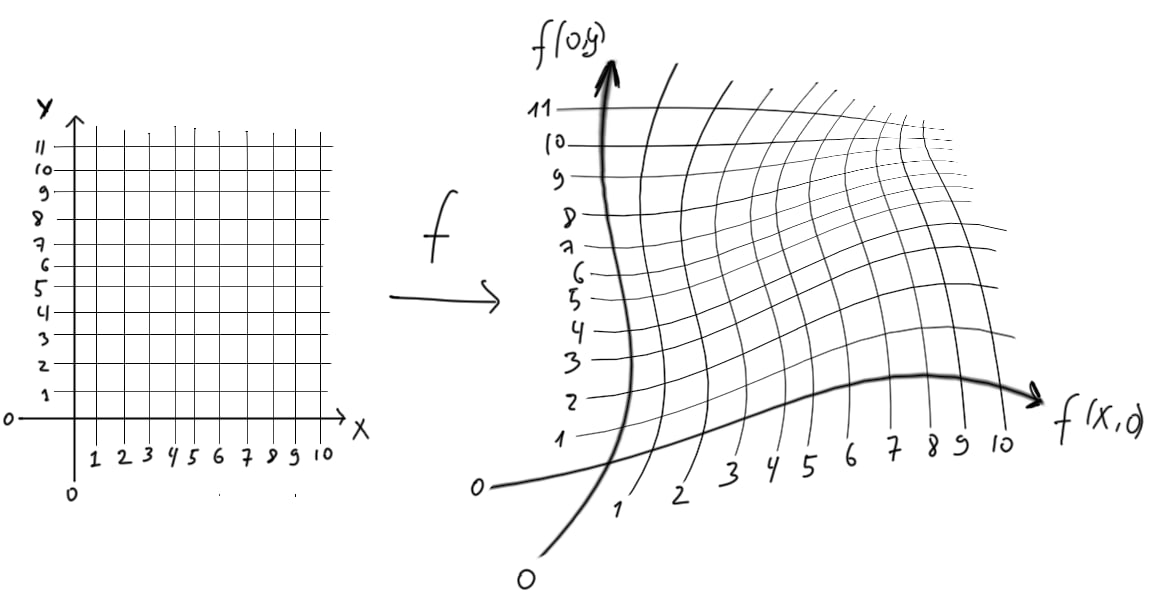
\includegraphics[scale =0.7]{deff2.jpg}
    \caption{Пример нелинейного отображения.}
    \label{deff2}
\end{figure}

Можно рассмотреть, например, и что-то более экзотическое, как показано на рисунке \ref{deff1}.

\begin{figure}
    \centering
    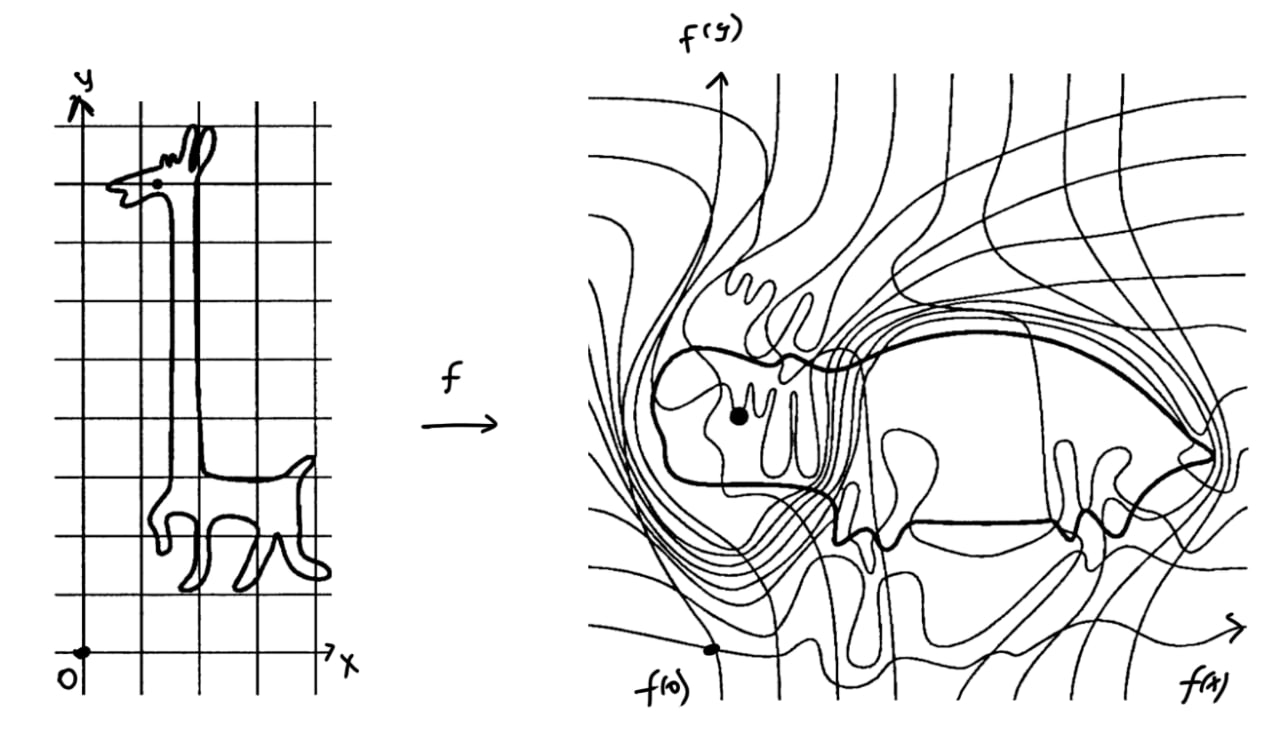
\includegraphics[scale = 0.5]{deff1.jpg}
    \caption{Пример нелинейного отображения: из жирафа получается бегемот.}
    \label{deff1}
\end{figure}

Однако же, это не означает, что линейную алгебру не надо изучать. Как раз наоборот, в сущности, анализ изучает любые подобное отображения с помощью линейной алгебры; локально они устроены как раз таки линейно (см. Рис.\ref{deff+linear}).

\begin{figure}
    \centering
    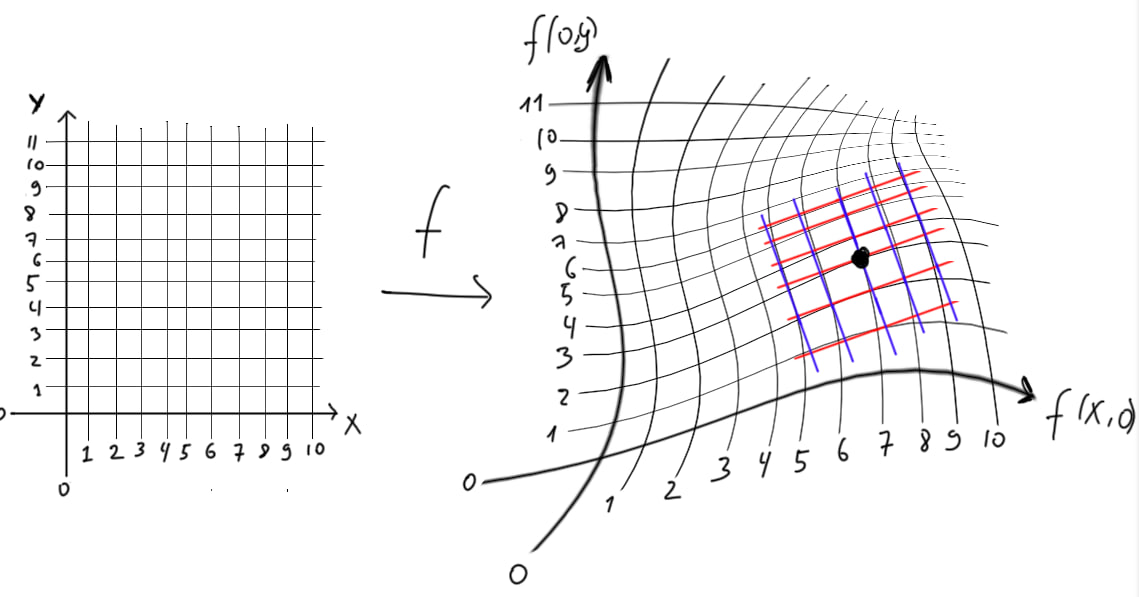
\includegraphics[scale = 0.7]{deff+linear.jpg}
    \caption{Вблизи это трудное отображение очень похоже на линейное.}
    \label{deff+linear}
\end{figure}




\section{Метрические пространства}

Определим \textit{метрическое пространство.} Пусть $E$ -- некоторое множество. \textit{Расстояние} в $E$ есть отображение $d:E\times E \to \mathbb{R}_{\ge 0}$, обладающее следующими свойствами:
\begin{enumerate}
    \item $d(x,y) = 0$, если и только если $x = y$.
    \item $d(x,y)=d(y,x)$, для любых $x,y \in E$.
    \item $d(x,z) \le d(x,y) + d(y,z)$, для любых трёх $x,y,z\in E$ (\textit{неравенство треугольника}).
\end{enumerate}

\subsection{Примеры расстояний}

 \begin{enumerate}
     \item Функция $d(x,y):=|x-y|$ есть расстояние в множестве $\mathbb{R}$ действительных чисел.
     \item В $\mathbb{R}^2$ обычное евклидово расстояние определяется формулой
     \[
       d(\m{x}, \m{y}):= \sqrt{(x_1 -y_1)^2 + (x_2 - y_2)^2},
     \]
     где $\m{x} = (x_1,x_2)$, $\m{y} = (y_1,y_2).$
     \item На плоскости $\mathbb{R}^2$ можно также ввести расстояние следующим образом:
     \[
      d(\m{x},\m{y}):= |x_1-y_1| + |x_2-y_2|.
     \]
     \item Ещё один пример расстояния на плоскости:
     \[
       d(\m{x},\m{y}):=\max\{|x_1 - y_1|, |x_2 - y_2|\}.
     \]
 \end{enumerate}

\subsection{Изометрия}~

Пусть $E,E'$ -- два метрических пространства, $d,d'$ -- расстояния в $E$ и $E'$. Биективное отображение $f:E \to E'$ называется \textit{изометрией}, если
\[
 d'(f(x), f(y)) = d(x,y)
\]
для любой пары элементов пространства $E$ обратное отображение $f^{-1}$ является изометрией пространства $E'$ на $E$. Два метрических пространства называются $E,E'$ \textit{изометричны}, если существует изометрия $E$ на $E'$.


Пусть $E$ -- метрическое пространство, $d$ -- расстояние в $E$ и $f$ -- биективное отображение $E$ на какое-то множество $E'$\footnote{в $E'$ до этого расстояние могло быть и не определено.} Мы можем тогда определить в $E'$ расстояние $d'$ как выше, \ie
\[
 d'(f(x), f(y)) = d(x,y),
\]
и в таком случае $f$ будет изометрией пространства $E$ в $E'$. Говорят, что расстояние $d'$ было \textit{перенесено} с $E$ на $E'$ отображением $f.$

\subsection{Расширенная действительная прямая $\overline{\mathbb{R}}$ и как измерять расстояние до бесконечности}~

Функция $f$, определённая на $\mathbb{R}$ условием 
\[
f(x) = \frac{x}{1+ |x|},
\]
является биективным отображением $f:\mathbb{R} \to (-1,1)$. Обратное отображение определяется формулой 
\[
 f^{-1}(x) = \frac{x}{1- |x|}
\]
при $|x|<1.$

Обозначим через $\overline{\mathbb{R}}$ множество, являющееся объединением $\mathbb{R}$ и двух новых элементов, обозначаемых символами $+\infty$ и $- \infty$ (=\textit{бесконечные точки}).

Тем самым, мы имеем вложение (инъекцию) $\mathbb{R} \hookrightarrow \overline{\mathbb{R}}$. Продолжим $f$ до биективного отображения $\overline{f}: \overline{\mathbb{R}} \to [0,1]$, полагая
\[
\overline{f}(x) = \begin{cases}
    f(x), & x \in \mathbb{R},\\
    1, & x = \infty,\\
    -1, & x = - \infty.
\end{cases}
\]

Тогда
\[
\overline{f^{-1}}(x) = \begin{cases}
    f^{-1}(x), & x \in (0,1),\\
    \infty, & x = 1,\\
    -\infty, & x = - 1.
\end{cases}
\]

Теперь мы можем ввести расстояние на $\overline{\mathbb{R}}$, $\overline{d}(x,y):=|\overline{f}(x) - \overline{f}(y)|$, $x,y \in \overline{\mathbb{R}}.$ Более подробно,
\begin{eqnarray*}
    \overline{d}(x,y) &=& \left| \frac{x}{1+|x|} - \frac{y}{1+|y|} \right|, \qquad x,y\in \mathbb{R}\\
    d(x, + \infty) &=& \frac{1}{1+|x|}, \qquad x \ge 0\\
    d(-\infty,x) &=& \frac{1}{1+|x|}, \qquad x \le 0.
\end{eqnarray*}

На $\overline{R}$ введём отношение порядка, по определению считая неравенство $x \le y$ эквивалентным неравенству $f(x) \le f(y)$. Легко проверить, что когда $x,y \in \mathbb{R}$, это отношение порядка есть обычное отношение порядка на $\mathbb{R}$ и что, кроме того, для любого $x\in \mathbb{R}$ мы имеем $- \infty < x < \infty.$

Действительные числа называются также \textit{конечными} элементами $\overline{\mathbb{R}}.$ 


\subsection{Шары и сферы}~

Элементы метрического пространства будем также называть \textit{точками}. 

\begin{definition}
    Пусть $E$ -- метрическое пространство с расстоянием $d$, а \textit{открытым шаром} (соотв. \textit{замкнутым шаром, сферой}) с центром в точке $a \in E$ и радиусом $r \in \mathbb{R}^+$ называется множество $B(a,r):=\{x\in E,\ |\, d(a,x)<r\}$ (соответственно, $\overline{B}(a,r):= \{x\in E\, |\, d(a,x) \le r\}$, $S(a,r):=\{x \in E\, |\, d(a,x) = r \}$).
\end{definition}

\begin{example}~
    \begin{enumerate}
        \item На действительной прямой $\mathbb{R}$ с расстоянием $d(x,y):=|x-y|$ имеем
        \[
         B(a,r) = (a-r, a+r), \qquad \overline{B}(a,r) = [a-r, a+r], \qquad S(a,r) = \{a-r, a+r\}.
        \]
        \item На расширенной прямой $\overline{\mathbb{R}}$ имеем
        \[
         B(+\infty, r) = \left(\frac{1-r}{r}, +\infty \left. \right. \right].
        \]
    \end{enumerate}
\end{example}


\subsection{Открытые множества и окрестности}~

\begin{definition}\label{def_of_open}
    \textit{Открытым множеством} в метрическом пространстве $E$ с расстоянием $d$ называется подмножество $A \subseteq E$, обладающее следующим свойством: для любой точки $x \in A$ существует такое $r >0$, что $B(x,r) \subseteq A$. Пустое множество открыто; всё пространство $E$ открыто. 
\end{definition}

\begin{lemma}\label{open_ball=open}
    Любой открытый шар в пространстве $E$ с расстоянием $d$ является открытым множеством.
\end{lemma}
\begin{proof}
    Пусть $B(a,r)$ -- открытый шар, по аксиоме выбора мы можем взять точку $x \in B(a,r)$, $x \ne a$. Тогда по определению $d(x,a) < r$. Рассмотрим теперь открытый шар $B(x,\delta)$, где $0 < \delta < r- d(a,x).$ Покажем, что $B(x,\delta ) \subseteq B(a, r)$, это и докажет лемму.

    По аксиоме выбора мы можем взять такое $y \in B(a,\delta)$, что $d(x,y)<\delta < r - d(a,x) $, тогда по неравенству треугольника
    \[
      d(a,y) \le d(a,x) + d(x,y) < d(a,x) + r - d(a,x) = r, 
    \]
    \ie $y\in B(a,r)$, что и доказывает $B(x,\delta) \subseteq B(a,r)$. Так как точка $x$ была выбрана произвольной в шаре $B(a,r)$, это показывает, что для любой точки в шаре мы нашли такой открытый шар, который целиком лежит в $B(a,r)$, \ie он открыт.
\end{proof}

\begin{lemma}\label{union_and_cap_of_open}
    Объединение любого семейства открытых множеств открыто и пересечение конечного числа открытых множеств открыто. 
\end{lemma}
\begin{proof}\
 
(1) Пусть $\mathscr{U} = \cup_{\alpha \in A}\mathscr{U}_\alpha$ и пусть $x \in \mathscr{U}$, тогда для какого-то $\alpha \in A$, $x \in \mathscr{U}_a$. Так как $\mathscr{U}_\alpha$ -- открыто, то найдётся такой $r >0$, что $B(x, r ) \subseteq \mathscr{U}_\alpha \subseteq \cup_{\alpha \in A}\mathscr{U}_\alpha$, что и доказывает открытость $\mathscr{U}.$

(2) Достаточно доказать, что множество двух открытых множеств $\mathscr{U}_1, \mathscr{U}_2$ открыто, а затем провести индукцию. Если $x \in \mathscr{U}_1 \cap \mathscr{U}_2$, то найдутся такие $r_1, r_2 >0$, что $B(x, r_1) \subseteq \mathscr{U}_1$, $B(x, r_2) \subseteq \mathscr{U}_2$. Очевидно, что $B(x, r) \subseteq \mathscr{U}_1 \cap \mathscr{U}_2$, где $r:= \min(r_1, r_2)$, что и доказывает открытость пересечения.
\end{proof}

\begin{definition}
    Пусть $A$ -- непустое множество в метрическом пространстве $E$ с расстоянием $d$. \textit{Открытой окрестностью} множества $A$ называется любое открытое множество $\mathscr{U}(A)$, содержащее $A$. В случае, когда $A = \{x\}$, мы говорим об окрестности $\mathscr{U}(x)$ точки $x$ (а не множества $\{x\}).$
\end{definition}

\begin{mydanger}{\bf{!}}
 Очевидно, что $\mathscr{U}(x)$ можно отождествить с подходящим открытым шаром $B(x,r)$, поэтому иногда мы не будем делать разницу между открытым шаром с центром в точке $x$ и открытым множеством, содержащим эту же точку $x.$    
\end{mydanger}

\subsection{Непрерывные отображения}

\begin{definition}
    Пусть $E$, $E'$ -- два метрических пространства, $d$ и $d'$ -- расстояния в них. Отображение $f:E \to E'$ называется \textit{непрерывным в точке $x_0 \in E$}, если для каждой окрестности $\mathscr{U}'$ точки $f(x_0) \in E'$ существует такая окрестность $\mathscr{U}(x_0)$ в $E$, что $f(\mathscr{U}(x_0)) \subseteq \mathscr{U}'(f(x_0))$. Отображение $f$ называется \textit{непрерывным в $E$} (или просто непрерывным), если оно непрерывно в каждой точке пространства $E.$
\end{definition}

Это же определение можно переформулировать и таким образом:

\begin{definition}
    Отображение $f:E \to E'$ непрерывно в точке $x_0$, если для любого шара $B(f(x_0), r) \subseteq E'$ всегда можно найти такой шар $B(x_0, \delta) \subseteq E$, что $f(B(x_0, \delta)) \subseteq B(f(x_0), r)$.
\end{definition}

Можно ещё вот так сказать:

\begin{definition}\label{reform_of_cont}
    Для того, чтобы отображение $f:E \to E'$ было непрерывно в точке $x_0 \in E$, необходимо и достаточно, чтобы для всякого $\varepsilon>0$ существовал такой $\delta >0$, что из $d(x_0,x)<\delta$ следует $d'(f(x),f(x_0))<\varepsilon$.
\end{definition}

\begin{figure}[h!]
    \centering
    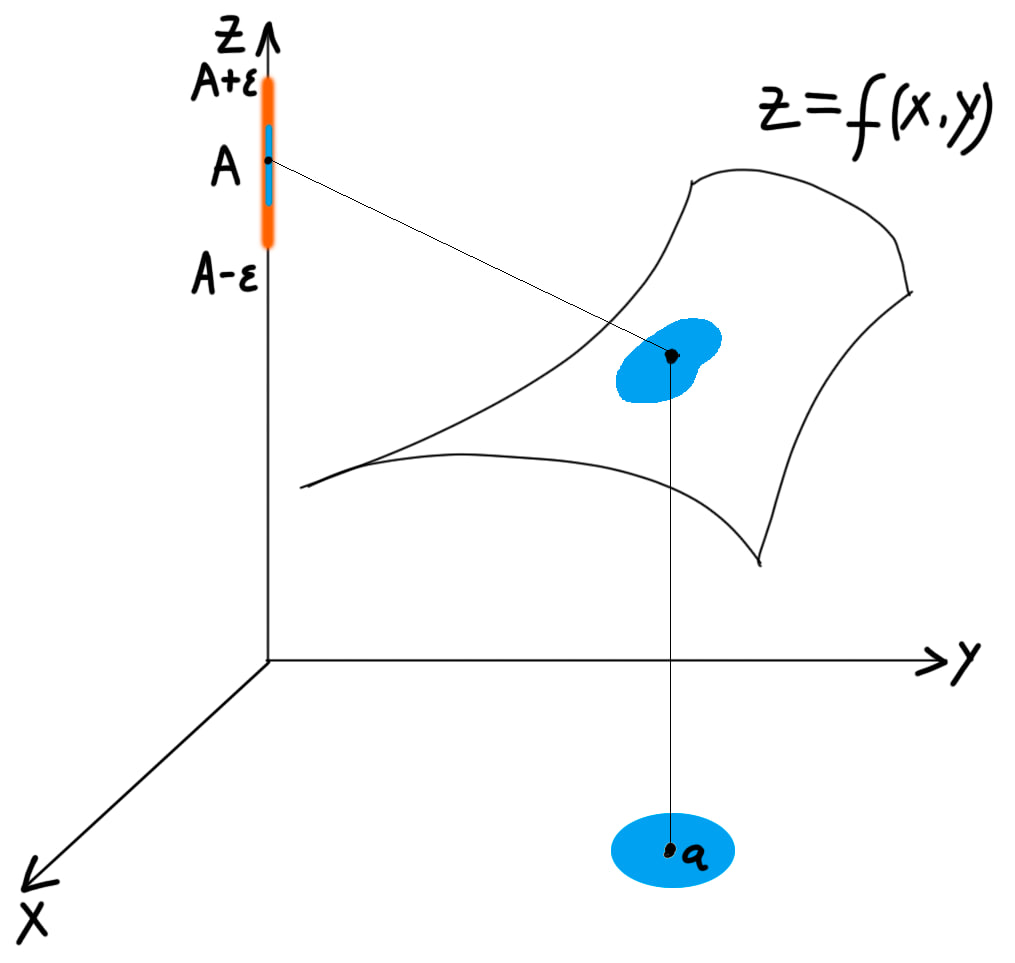
\includegraphics[scale=0.5]{continous3.jpg}
    \caption{График отображения $f: \mathbb{R}^2 \to \mathbb{R}$ есть некоторая поверхность в $\mathbb{R}^3$. Нужно понимать, что мы горизонтальную плоскость отображаем в вертикальную прямую. Здесь показано, почему в точке $\m{a}\in \mathbb{R}^2$ это отображение непрерывно, $f(\m{a}) = A$. Какой бы оранжевый шар $\textcolor{orange}{B(A, \varepsilon)} \subseteq \mathbb{R}$ мы не взяли, можно найти синий шар $\textcolor{blue}{B(\m{a},r)} \in \mathbb{R}^2$ такой, что его образ $f( \textcolor{blue}{B(\m{a}, r)} )$ в вертикальной прямой (синяя полоска в оранжевом отрезке) будет целиком содержаться в этом оранжевом шаре.}
    \label{fig:enter-label}
\end{figure}


\begin{remark}\label{not_continous}
    Тогда если $f(x)$ не является непрерывным в точке $x_0$, то какой бы шар $B(x_0, \delta) \subseteq E$ мы не выбрали, всегда можно найти такой шар $B(f(x_0),r)$, что $f(x) \notin B(f(x_0),r)$ для каких-то $x \in B(x_0, \delta).$
\end{remark}


\begin{example}\label{x^2sin(1x)}
    Пусть $E = E' = \mathbb{R}$ с одинаковой метрикой $d(x,y) = |x-y|$, покажем, что отображение $\overline{f}:E \to E'$;
    \[
     \overline{f}(x) = \begin{cases}
         x^2 \sin \frac{1}{x}, & x \ne 0, \\
         0, & x =0
     \end{cases}
    \]
    непрерывно в точке $0$.

    Это значит, что для любого $\varepsilon >0$ мы должны найти такую $\delta >0$, что из неравенства $|x|<\delta$ будет следовать $|\overline{f}(x) - \overline{f}(0)| <\varepsilon.$ Чтобы найти такую $\delta$, мы заметим, что 
    \[
    \left|\overline{f}(x) -\overline{f}(0)\right| = \left|x^2 \sin \frac{1}{x} - 0 \right| = \left|x^2 \sin \frac{1}{x}\right| \le |x^2| = x^2,
    \]
поэтому если $x^2 <\varepsilon$, \ie $-\sqrt{ \varepsilon} <x < \sqrt{\varepsilon}$, то и $|\overline{f}(x) - \overline{f}(0)| <\varepsilon$. Значит, для любого $0 < \delta < \sqrt{\varepsilon}$ из неравенства $|x|<\delta$ вытекает неравенство $|\overline{f}(x) - \overline{f}(0)|$, что и доказывает непрерывность в точке $0.$
\end{example}

\begin{theorem}\label{preimage_of_open}
    Отображение $f:E \to E'$ между метрическими пространствами непрерывно тогда и только тогда, когда прообраз любого открытого в $E'$ открыт в $E.$
\end{theorem}
\begin{proof}~

(1) Пусть $f:E \to E'$ непрерывно. Возьмём открытое $\mathscr{U}' \subseteq E'$ и покажем, что $\mathscr{U}:=f^{-1}(\mathscr{U'})$ открыто в $E$. Пусть $x \in \mathscr{U}$, тогда $f(x) = x' \in \mathscr{U}'$, так как $\mathscr{U}'$ -- открыто в $E'$, то найдётся шар $B'(x',r') \subseteq \mathscr{U}'$. Так как шар $B'(x',r')$ есть открытая окрестность точки $x'$ и по предположению $f$ непрерывна и в точке $x \in E$, значит, найдётся такой шар $B(x,r) \subseteq E$ такой, что $f(B(x,r)) \subseteq B'(x',r')$. 

Таким образом, мы имеем $f(B(x,r)) \subseteq B'(x',r') \subseteq \mathscr{U}' .$ С другой стороны, если $A'\subseteq B' \subseteq E'$, то ясно, что $f^{-1}(A') \subseteq f^{-1}(B')$. Действительно, по определению прообраза
    \[
     f^{-1}(A'):= \{x \in X\, |\, f(x) \in A' \subseteq B'\} \Longrightarrow f^{-1}(A') \subseteq f^{-1}(B').
    \]

 Итак, мы получили, что $f(B(x,r)) \subseteq B'(x',r') \subseteq \mathscr{U}'$, тогда
 \[
  f(B(x,r)) \subseteq \mathscr{U}' \Longleftrightarrow f^{-1}(f(B(x,r))) \subseteq f^{-1}(\mathscr{U}')  \Longleftrightarrow B(x,r) \subseteq \mathscr{U},
 \]
 \ie для любого $x \in \mathscr{U}$ мы нашли шар $B(x,r)$, который целиком находится в $\mathscr{U}$, а это и означает, что $\mathscr{U}$ открыто.

(2) Пусть прообраз любого открытого есть открытое множество в $E.$ Пусть $\mathscr{U}'$ -- открытое в $E'$. Аксиома выбора позволяет нам выбрать точку $x' \in \mathscr{U}'$. Тогда для произвольно выбранной точки $x'$ существует такой открытый шар $B'(x',r')$, что $B'(x',r') \subseteq \mathscr{U}'.$

Пусть $f(x) = x'$, \ie $x \in f^{-1}(B'(x',r'))$. По предположению $f^{-1}(B'(x',r'))$ открыто в $E$. Это значит, что для любой выбранной точки $y \in f^{-1}(B'(x',r'))$ можно найти такой открытый шар $B(y,r)$, что $B(y,r) \subseteq f^{-1}(B'(x',r'))$. В частности, $B(x,r) \subseteq f^{-1}(B'(x',r'))$ 

Вспоминая, что если $A \subseteq B$, то и $f(A) \subseteq f(B)$. Тогда получаем 
\[
  B(x,r) \subseteq f^{-1}(B'(x',r')) \Longrightarrow f(B(x,r)) \subseteq f(f^{-1}(B'(x',r'))) \subseteq B'(x',r'),
\]
\ie для любого открытого шара $B'(x',r')$, где $x' = f(x)$, мы нашли такой открытый шар $B(x,r)$, что $f(B(x,r)) \subseteq B'(x',r')$, но это и означает непрерывность.
\end{proof}

\begin{corollary}
    Отображение $f:E \to E'$ -- непрерывно в точке $x$, тогда и только тогда, когда прообраз любого открытого шара $B(f(x),r) \subseteq E'$ -- открытое множество в $E$
\end{corollary}
\begin{proof}
    Это сразу следует из предыдущей теоремы и леммы \ref{union_and_cap_of_open}.
\end{proof}

\begin{theorem}\label{comp_of_continous}
    Пусть $E,E,E''$ -- метрические пространства и пусть $f:E \to E'$, $g:E' \to E''$ -- отображения. Если $f$ непрерывно в точке $x_0$ и $g$ непрерывно в $f(x_0)$, то $h = g \circ f$ непрерывно в точке $x_0.$ Если $f$ непрерывно в $E$ и $g$ непрерывно в $E'$, то $h$ непрерывно в $E.$
\end{theorem}
 \begin{proof}
     Второе утверждение, очевидно, следует из первого. Пусть $\mathscr{U}''$ -- окрестность точки $h(x_0) =  g(f(x_0))$. Тогда из предположения о непрерывности и Теоремы \ref{preimage_of_open} следует, что $\mathscr{U}':=g^{-1}(\mathscr{U}'')$ -- открытое множество в $E'$, содержащее точку $f(x_0)$. Далее, так как $f$ непрерывно, то по теореме \ref{cap_of_intervals}, прообраз $\mathscr{U}:=f^{-1}(\mathscr{U}')$ -- открытое множество, содержащее точку $x_0$. Таким образом, $h^{-1}(\mathscr{U}'') = \mathscr{U}$ открытое, тогда по теореме \ref{preimage_of_open}, $h$ непрерывно в точке $x_0$, что и завершает доказательство. 
 \end{proof}


\begin{corollary}\label{restriction}
    Если $f$ -- отображение метрического пространства $E$ в метрическое пространство $E'$, непрерывное в точке $x_0$, и $A \subseteq E$, $A \ni x_0$, то сужение $f|_A:=f \circ \mathrm{in}_A$ также непрерывно в $x_0,$ где $\mathrm{in}_A:A \hookrightarrow E$ -- вложение.
\end{corollary}
\begin{proof}
    На самом деле, $f$ непрерывно в $x_0$ по условию, а $\mathrm{in}_A$ непрерывно в любой точке $a \in A$, тогда из предыдущей теоремы и следует утверждение.
\end{proof}

 \begin{remark}\label{+infty}
    Пусть $E = \overline{\mathbb{R}}$ -- расширенная прямая, рассмотрим выражение $\lim_{x \to +\infty, x \in \mathbb{{R}}}f(x) = a'$, где $f:\mathbb{R} \to E' $ -- некоторое отображение. Мы знаем, что $B(+\infty, \delta) = (\frac{1-\delta}{\delta}, \infty]$. Тогда непрерывность в точке $+\infty$ означает, что для любого $r >0$ найдётся такая $\delta>0$, что $f((\frac{1-\delta}{\delta}, \infty]) \subseteq B(a',r)$. Другими словами, для любого шара $B(a',r)$ найдётся такое число $\alpha \in \mathbb{R}$, что $f(\beta) \in B(a',r)$ для всех $\beta > \alpha.$
\end{remark}

\section{Замкнутые множества, точки замыкания (=точки прикосновения), замыкание множества.}

\begin{definition}
    \textit{Замкнутое множество} в метрическом пространстве $E$ есть дополнение открытого множества. 
\end{definition}

Пустое множество замкнуто, замкнуто и всё пространство $E$.

\begin{example}
    Пусть $E = \mathbb{R}$, $d(x,y):= |x-y|$. Тогда промежутки $[a, + \infty)$, $(- \infty,a]$ замкнуты, потому что 
    \[
     [a, + \infty) = \mathbb{R} \setminus \cup_{n \ge 1} (a-n, a)
    \]
\end{example}





\begin{definition}\label{limit_point_in_metric}
  Пусть $E$ -- метрическое пространство, $d$ -- расстояние в нём, и пусть $A \subseteq E$. \textit{Точка замыкания} (=\textit{точка прикосновения}) множества $A$ -- такая точка $x \in E$, каждая окрестность которой имеет с $A$ непустое пересечение. Множество всех точек замыкания называется \textit{замыканием} множества $A$ и обозначается символом $\overline{A}.$
\end{definition}

\begin{example}~
    \begin{enumerate}
        \item $E= \mathbb{R}$ с обычной метрикой $d(x,y) = |x-y|$, $A = (0,1]$, тогда $0$ -- точка замыкания, потому что любой шар $B(0,r) = (-r,r) \cap A \ne \varnothing$.
        \item На расширенной прямой $\overline{\mathbb{R}}$ шары $B(+\infty, r) = (\frac{1-r}{r}, +\infty)$ есть просто луч. Ясно, что $B(+\infty, r)\cap \mathbb{R} \ne \varnothing$, \ie это и означает, что замыкание множества $\mathbb{R}$ и даст расширенную прямую $\overline{\mathbb{R}}.$
    \end{enumerate}
\end{example}

\begin{lemma}\label{closure_in_metric}
    Множество $F$ в метрическом пространстве замкнуто, если и только если все его точки это предельные точки, \textit{т.е.,} $F = \overline{F}.$ 
\end{lemma}
(1) Пусть $F$ -- замкнуто, тогда найдётся какое-то открытое $\mathscr{U} \subseteq E$, такое, что $F  = E \setminus \mathscr{U}$. Пусть $x \notin F$, тогда $x \in \mathscr{U}$, и тогда найдётся окрестность $\mathscr{W}(x)$ такая, что $\mathscr{W}(x) \subseteq \mathscr{U}$, потому что $\mathscr{U}$ -- открыто, \textit{т.е.,} $\mathscr{W}(x) \cap F = \varnothing.$ Таким образом, получили, что если $F$ -- замкнуто, то никакая точка $x \notin F$ не может быть предельной для $F$, \textit{т.е.,} $F = \overline{F}.$ 

(2) Пусть $F = \overline{F}$, тогда для любой точки $x \notin F$, можно всегда найти окрестность $\mathscr{W}(x)$ такую, что $\mathscr{W}(x) \cap F = \varnothing$. Пусть $\mathscr{U}:= \cup_{x E\setminus F} \mathscr{W}(x)$, тогда, $\mathscr{U}$ -- открыто в $E$ и $F = E \setminus \mathscr{U}.$


\begin{lemma}\label{preimage_of_closed}
    Отображение $f:E \to E'$ между метрическими пространствами непрерывно тогда и только тогда, когда прообраз любого замкнутого множества в $E'$ есть замкнутое множество в $E.$
\end{lemma}

\begin{proof}
    Пусть $F'$ -- замкнутое подмножество в $E'$, тогда $\mathscr{U}': = E'\setminus F'$ -- открыто в $E'$ и $E' = F' \cup \mathscr{U}'$, $F' \cap \mathscr{U}' = \varnothing$. Далее, ясно что $f^{-1}(F') \cap f^{-1}(\mathscr{U}') = \varnothing$ и $E = f^{-1}(F') \cap f^{-1}(\mathscr{U}')$. Тогда согласно Теореме \ref{preimage_of_open}, $f$ -- непрерывно если и только если $f^{-1}(\mathscr{U}')$ -- открыто в $E$, но тогда $f^{-1}(F') = E \setminus \mathscr{U}'$ замкнуто тогда и только тогда, когда $f^{-1}(\mathscr{U}')$ -- открыто. Это завершает доказательство.
\end{proof}

\begin{lemma}\label{closed_ball=closed}
    Замкнутый шар -- замкнут.
\end{lemma}
\begin{proof}
Пусть $(E,d)$ -- метрическое пространство, $\bar B(a,r)$ -- замкнутый шар. Покажем, что $E\setminus B(a,r)$ -- открыто. Пусть $x\notin \bar B(a,r)$, тогда $d(a,x) > r$, и положим $\varepsilon: = d(a,x) - r$, очевидно, что $\varepsilon >0$. Имеем $d(x,a) \le d(y,a) + d(y,x)$, тогда $d(y,a) \ge d(x,a) - d(y,x)$.

Пусть теперь $y\in B(x, \frac{\varepsilon}{2})$, тогда получаем
\begin{eqnarray*}
    d(y,a) &\ge & d(x,a) - d(y,x) \\
    &\ge & r + \varepsilon- \frac{\varepsilon}{2}\\
    &=& r + \frac{\varepsilon}{2}\\
    &>& r
\end{eqnarray*}
\textit{т.е.,} $y\notin \bar B(a,r)$. А это означает, что весь открытый шар $B(x, \frac{\varepsilon}{2})$ не лежит в $\bar B(a,r)$, что и требовалось доказать.
\end{proof}



\section{Подпространства метрического пространства}

Пусть $F \subseteq E$ -- непустое подмножество метрического пространства $E$ с расстоянием $d$, тогда $F \times F \subseteq E \times E$ -- непустое подмножество, тогда мы имеем следующую коммутативную диаграмму

\[
  \begin{tikzcd}
    F \times F \arrow[hook]{d}[left]{\mathrm{in}} \arrow{dr}{d|_{F \times F}} &  \\
    E \times E \arrow{r}[below]{d} & \mathbb{R}
  \end{tikzcd}
\]
\ie, \textit{сужая} метрику $d$ на $F$, мы получаем метрическое пространство $(F,d|_{F \times F})$, которое мы будем для простоты обозначать $(F, d_F)$.

\begin{definition}
    Метрическое пространство, определённое таким образом, называется \textit{подпространством} $F$ метрического пространства $E$.
\end{definition}

\begin{figure}[h!]
    \centering
    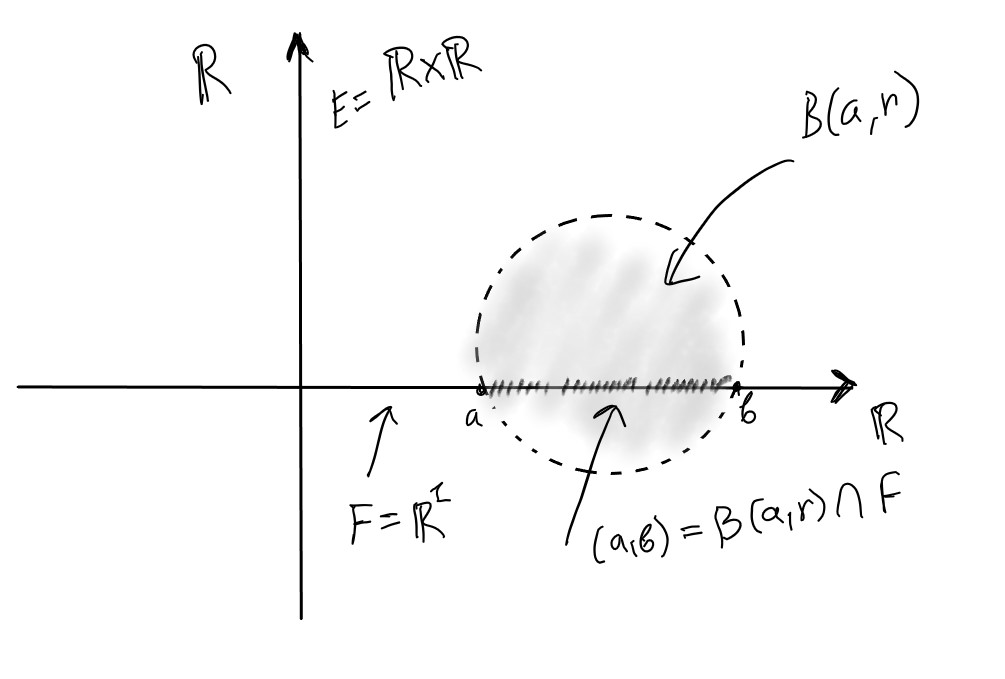
\includegraphics[scale = 0.4]{open_in_F.jpg}
    \caption{Пусть $E = \mathbb{R} \times \mathbb{R}$ -- обыкновенная плоскость с обыкновенной евклидовой метрикой $d(\m{x},\m{y}) = \sqrt{(x_1 - y_1)^2+ (x_2 - y_2)^2}$, и пусть $F = \mathbb{R}$, которую мы можем понимать как множество вида $\{(x,0), x\in \mathbb{R}\}$. На рисунке $F$ отождествлена с осью $Ox$. Тогда, сужая метрику $d$ на $F$, мы получаем, что $d(x,y) = \sqrt{(x-y)^2} = |x-y|$. Более того, ясно, что любой интервал $(a,b)$ можно получить, пересекая открытый круг с $F.$}
    \label{fig:enter-label}
\end{figure}


\begin{proposition}\label{open_in_subset}
    Для того чтобы множество $S \subseteq F$ было открыто в подпространстве $F$, необходимо и достаточно, чтобы существовало такое множество $\mathscr{U}$, открытое в $E$, что $S = \mathscr{U} \cap F.$
\end{proposition}

\begin{proof}
    Прежде всего, поймём, что есть открытый шар в $F$. Пусть $a \in F$, и рассмотрим открытый шар $B(a,r) \subseteq E$, тогда получаем
    \begin{eqnarray*}
        F \cap B(a,r) &:=& \{x \in E \cap F\, :\, d(x,a)<r\} \\
        &=&\{x\in F\, :\, d(x,a)<r\} \\
        &=& \{x \in F\, :\, d_F(x,a)<r\},
    \end{eqnarray*}
    \ie $F \cap B(a,r)$ -- это \textbf{открытый шар в $F$ с центром в точке $a$ радиуса $r.$}

\begin{mydanger}{\bf{!}}
    Обратим внимание, что если $F = \mathbb{R}_{\ge 0} \subseteq \mathbb{R} = E$, $d(x,y) = |x-y|$, то, например, $[0,1)$ -- открытый шар в $F = \mathbb{R}_{\ge 0}$, так как $[0,1) = (-1,1) \cap \mathbb{R}_{\ge 0}$. Hо! В $\mathbb{R}$, $[0,1)$ и не открыт и не замкнут!
\end{mydanger}

(1) Пусть $\mathscr{U}$ -- открытое множество в $E$, и пусть $x \in \mathscr{U} \cap F$. Так как $\mathscr{U}$ -- открытое в $E$, то найдётся шар $B(x,r) \subseteq E$ такой, что $B(x,r) \subseteq \mathscr{U}$. Тогда $F \cap B(x,r) \subseteq F \cup \mathscr{U}$. Но мы уже поняли, что $B(x,r) \cap F$ -- открытый шар в $F$, но тогда включение $F \cap B(x,r) \subseteq F \cup \mathscr{U}$ и означает, что $\mathscr{U} \cap F$ открыто в $F$, ибо $x$ -- произвольная точка в $\mathscr{U} \cap F.$

(2) Пусть $S$ открыто в $F$, это значит, что для любой точки $x \in S$ можно найти открытый шар $B(x, r(x)) \subseteq E$ такой, что $F \cap B(x,r(x)) \subseteq S$ (т.к., $F \cap B(x,r(x))$ -- это открытый шар в $F$).

Тогда 
\[
 S = \bigcup_{x \in S} F \cap B(x, r(x)) = F \cap \mathscr{U},
\]
где $\mathscr{U} = \cup_{x\in S} B(x, r(x)) \subseteq E$, тогда по Леммам \ref{open_ball=open}, \ref{union_and_cap_of_open} $\mathscr{U}$ открыто в $E$.
\end{proof}

\section{Пределы}

Пусть $E$ -- метрическое пространство, $d$ -- расстояние в нём, пусть $A \subseteq E$ -- некоторое его подмножество, пусть $a$ -- точка замыкания для $A$, \ie $a \in \overline{A}$, и пусть $f:A \to E'$ некоторое отображение в метрическое пространство $E'.$

\begin{definition}\label{the_main_def_of_limit}
    Пусть $a \notin A$. Мы будем говорить, что $f(x)$ \textit{имеет предел $a' \in E'$ при $x \in A$, стремящемся к $a$ (или $a'$ есть предел отображения $f$ в точке $a\in \overline{A}$ по множеству $A$}), если отображение $\overline{f}:A \cup \{a\} \to E$, определённое условиями
    \[
     \overline{f}(x) = \begin{cases}
         f(x), & x \in A, \\
         a', & x = a,
     \end{cases}
    \]
    непрерывно в точке $a$.
\end{definition}

В этом случае, мы пишем
\[
 a' := \lim_{x\to a, x \in A} f(x).
\]

\begin{mydanger}{\bf{!}}
    Если $a \in A$, то мы пользуемся той же терминологией и теми же обозначениями как и в случае, когда отображение $f$ непрерывно в точке $a$, причём $a':=f(a).$
\end{mydanger}

\begin{example}~

 \begin{enumerate}
  \item Пусть $E = E'=\mathbb{R}$, $d(x,y) = d'(x,y): |x-y|$, $A = \mathbb{R}\setminus \{0\}$, и отображение $f: A \to \mathbb{R}$ задаётся с помощью $f(x) = x$. 

  Ясно, что $0$ есть точка замыкания для $A$, так как шар $B(0,r)$ с такой метрикой $d$ -- это просто интервал $(-r,r)$, тогда очевидно, что $(-r, r) \cap A = (-r, r)\setminus \{0\} \ne \varnothing$, что и доказывает, что точка $0$ -- точка замыкания для множества $A$.

  Пусть
  \[
   \overline{f}(x): = \begin{cases}
       x, & x \in A \\
       \alpha, & x =0.
   \end{cases}
  \]

Если мы поймём, при каком $\alpha$ это отображение $\overline{f}$ непрерывно в точке $0$, то мы и найдём предел, который и будет равен этому $\alpha.$

Итак, пусть $\overline{f}$ непрерывна в точке $0$, тогда для любого шара $B(\alpha, r) \subseteq E' = \mathbb{R}$ должен найтись шар $B(0,\delta) \subseteq E = \mathbb{R}$ такой, что $f(B(0,\delta)) \subseteq B(\alpha, r)$.

Ясно, что $B(0,\delta) = (-\delta, \delta)$, $B(\alpha, r) = (\alpha - r,\alpha + r)$, и 
\[
 \overline{f}(B(0,\delta)) = \overline{f}((-\delta, \delta)) = (-\delta, \delta) \setminus \{0\} \cup \{\alpha\},
\]
следовательно, если $\overline{f}$ будет непрерывной в точке $0$, то для любого $r >0$ можно найти $\delta >0$ такое, что
\[
 \overline{f}(B(0,\delta)) = (-\delta, \delta) \setminus \{0\} \cup \{\alpha\} \subseteq (\alpha - r, \alpha + r),
\]
тогда $-\delta, \delta \in (\alpha - r, \alpha + r)$. Это значит, что $\alpha -r < 0$, $\alpha + r >0$. Таким образом, если $\alpha \ne 0$, \textbf{то только для шаров вида (\ie не для всех!) $B(\alpha, r)$, где $\alpha -r < 0$, $\alpha + r >0$,} всегда найдётся шар $B(0,\delta)$ такой, что $f(B(0,\delta)) \subseteq B(\alpha, r)$, \ie при $\alpha \ne 0$ отображение $\overline{f}$ не будет непрерывным в $0$. С другой стороны, если же $\alpha =0$, то мы получаем неравенства $-r <0$, $r>0$, которые выполняются всегда, так как мы требуем чтобы $r>0$.

Таким образом, $\lim_{x\in 0, x \in A}f(x) = 0.$

 \item Пусть $E = E' = \mathbb{R}$ с расстоянием $d(x,y) = |x-y|$, $A = \mathbb{R}\setminus \{0\}$, $f(x): = x^2 \sin \frac{1}{x}.$ Тогда, как мы уже видели в примере \ref{x^2sin(1x)}, отображение  
     \[
     \overline{f}(x) = \begin{cases}
         x^2 \sin \frac{1}{x}, & x \ne 0, \\
         0, & x =0
     \end{cases}
    \]
    непрерывно в точке $x = 0$, тогда $\lim_{x \to 0, x \in A}f(x) = 0.$
 \end{enumerate}
    
\end{example}

Вспомнив определение непрерывности и точки замыкания, определение предела можно переформулировать следующими двумя эквивалентными способами:

\begin{definition}
    $\lim_{x \to a, x \in A}f(x) = a'$ эквивалентно тому, что для любого шара $B(a',r) \subseteq E'$ найдётся такой шар $B(a,\delta) \subseteq A$, что $f(B(a,\delta)\cap A) \subseteq B(a',r)$.
\end{definition}
\begin{mydanger}{\bf{!}}
    Так как $a$ -- точка замыкания, то множество $A \cap B(a,\delta)$ никогда не пусто для любого $\delta >0$.
\end{mydanger}




































\begin{definition}\label{def_for_cont_via_d-e}
    $\lim_{x \to a, x \in A}f(x) = a'$ эквивалентно тому, что для каждого $\varepsilon>0$ можно найти такое $\delta >0$, что из $x \in A$ и $d(x,a)<\delta$ следует $d'(a',f(x))<\varepsilon.$
\end{definition}

\begin{proposition}
    Отображение может иметь лишь один предел по множеству $A$ в данной точке $a \in \overline{A}.$
\end{proposition}
\begin{proof}
    Пусть  $\lim_{x \to a, x \in A}f(x) = a'$ и  $\lim_{x \to a, x \in A}f(x) = b'$, при этом $a' \ne b'$. Тогда, согласно Определению \ref{def_for_cont_via_d-e}, 
 \begin{enumerate}
     \item  $\lim_{x \to a, x \in A}f(x) = a'$ означает, что для любого $\varepsilon >0$ можно найти такое $\delta_1 >0$, что из $x \in A$ и $d(x,a)<\delta_1$ следует $d'(a',f(x))<\varepsilon$
     \item $\lim_{x \to a, x \in A}f(x) = b'$ означает, что для того же $\varepsilon >0$ можно найти такое $\delta_2 >0$, что из $x \in A$ и $d(x,a)<\delta_2$ следует $d'(b',f(x))<\varepsilon$.
 \end{enumerate}
Тогда по неравенству треугольника
\[
 d'(a',b') \le d'(a', f(x)) + d'(f(x), b') < 2\varepsilon,
\]
\ie расстояние между фиксированными точками $a',b' \in E'$ может быть любым, что невозможно если $a' \ne b'.$
\end{proof}

Из определения предела вытекает:
\begin{theorem}[{Критерий непрерывности}]\label{criteria_of_continous}
    Пусть $f$  -- отображение метрических пространств $f:E \to E'$. Для того чтобы $f$ было непрерывно в точке $x_0 \in E$, являющейся точкой замыкания множества $E\setminus\{x_0\}$, необходимо и достаточно, чтобы $f(x_0) = \lim_{x \to x_0, x\in E \setminus \{x_0\}}f(x).$
\end{theorem}
\begin{proof}
    Это лишь пересказ определения.
\end{proof}

\begin{theorem}\label{limit_for_any_subset}
    Пусть $a' = \lim_{x \to a, x \in A} f(x)$. Тогда для каждого подмножества $B \subseteq A$, для которого $a \in \overline{B}$, $a' = \lim_{x \to a, x \in B}f(x)$.
\end{theorem}

\begin{proof}
    Это сразу следует из определения предела и следствия \ref{restriction}.
\end{proof}

\begin{theorem}\label{lim_of_composition}
    Пусть $E,E',E''$ -- метрические пространства, $A \subseteq E$, и $f:A \to E'$, $g:E' \to E''$ -- отображения. Если $\lim_{x \to a, x \in A}f(x) = a'$ и $g$ непрерывно в точке $a'$, то $g(a') = \lim_{x \to a, x \in A}g(f(x))$. 
\end{theorem}
\begin{proof}
    Это сразу следует из определения предела и теоремы \ref{comp_of_continous}.
\end{proof}

\begin{mydanger}{\bf{!}}
    В случае, когда $A = E$, мы будем вместо $\lim_{x \to a, x \in A}f(x)$  писать $\lim_{x \to a}f(x).$
\end{mydanger}

\begin{remark}
 Пусть $E = \overline{\mathbb{R}}$ -- расширенная прямая, рассмотрим выражение $\lim_{x \to +\infty, x \in \mathbb{{R}}}f(x) = a'$, где $f:\mathbb{R} \to E' $ - некоторое отображение. Мы знаем, что $B(+\infty, \delta) = (\frac{1-\delta}{\delta}, \infty]$. Тогда непрерывность в точке $+\infty$ означает, что для любого $r >0$ найдётся такой $\delta>0$, что $f((\frac{1-\delta}{\delta}, \infty]) \subseteq B(a',r)$. Другими словами, если $\lim_{x \to + \infty} f(x) = a'$, то для любого шара $B(a',r)$ найдётся такое число $\alpha \in \mathbb{R}$ что $f(\beta) \in B(a',r)$ для всех $\beta > \alpha.$ \textbf{Именно так мы и будем понимать запись $\lim_{x \to +\infty}f(x) = a'$};
 \[
  \boxed{ 
    \boxed{
    \lim_{x \to +\infty}f(x) = a' \Longleftrightarrow \forall r > 0\, \exists \alpha \in \mathbb{R}:\, f(\beta) \in B(a',r) \,\forall \beta >\alpha.
    }
}
 \]
\end{remark}

\begin{mydanger}{\bf{!}}
    В частности, если $E' = \mathbb{R}$ с обычной метрикой и $\mathbb{N} \subseteq \overline{\mathbb{R}}$, то $\lim_{x \to +\infty, x \in \mathbb{{N}}}f(x) =a'$ есть знакомое нам определение предела последовательности.
\end{mydanger}

\begin{lemma}\label{choice_of_seqeunce}
    Для любой точки $a \in \overline{A}$ существует такая последовательность $\{x_n\}$ точек из $A$, что $a = \lim_{n \to \infty} x_n$
\end{lemma}

\begin{proof}
    Так как $a$ -- точка замыкания, то любой шар $B(a, r)$ содержит хотя бы одну точку из $A$, \ie $B(a, r) \cap A \ne \varnothing$. В частности, для любого $n\ge 1$, $B(a, \frac{1}{n}) \cap A \ne \varnothing$. Тогда по Аксиоме Выбора, для каждого $n\ge 1$ мы можем выбрать $x_n \in B(a, \frac{1}{n})$. Покажем, что $\lim_{n \to \infty} x_n = a$. Действительно, пусть $n<m$, и мы имеем тогда $x_n \in B(a, \frac{1}{n})$, $x_m \in B(a, \frac{1}{m})$. 

    Тогда имеем
    \[
     d(x_n, x_m) \le d(a,x_n) + d(a,x_m) <\frac{1}{n} + \frac{1}{m} < \frac{2}{n}.
    \]

Это означает, что все $x_n, x_{n+1}, \ldots \in B(a, \frac{2}{n})$, что и доказывает требуемое.
\end{proof}

\begin{corollary}\label{Weirstrass_mega}
    Подмножество $F$ в метрическом пространстве $E$ замкнуто, тогда и только тогда, когда из любой последовательности $(x_n)$ в $F$, можно выбрать сходящуюся подпоследовательность $(x_{n_k})$, такую, что $\lim_{n\to \infty} x_{n_k} \in F$. 
\end{corollary}

\begin{proof}
    По Предложению \ref{closure}, $F$ замкнуто, если и только если $F = \overline{F}$. Тогда используя лемму \ref{choice_of_seqeunce}, мы завершаем доказательство. 
\end{proof}



\begin{theorem}\label{lim=>for_any_sequence}
    Пусть $f: A \to E'$ -- отображение множества $A \subseteq E$ в метрическое пространство $E'$ и $a \in \overline{A}.$ Для того, чтобы $f$ имело предел $a' \in E'$ в точке $a$ по $A$, необходимо и достаточно, чтобы для каждой последовательности $\{s_n\}$ точек из $A$, сходящейся к $a$, последовательность $f(s  _n)$ сходилась к $a'.$
\end{theorem}

\begin{proof}~

(1) Необходимость. 

Пусть $\lim_{x \to a, x \in A}f(x) = a'$, и пусть $s:\mathbb{N} \to {A}\cup \{a\}$ -- последовательность $\{s_n\}$. По условию, $\lim_{n \to \infty }s_n = a$ и так как $\lim_{x \to a, x \in A}f(x) = a'$, то по определению предела \ref{the_main_def_of_limit}, $\overline{f}$ непрерывна в точке $a$. Тогда по Теореме \ref{lim_of_composition}, последовательность $s':=\overline{f} \circ s: \mathbb{N} \to E'$, в которой $s'_n = f(s_n)$, имеет предел $\overline{f}(a) = a'$, что и доказывает необходимость.

(2) Достаточность.

Будем доказывать от противного. Пусть для любой последовательности $\{s_n\}$ точек из $A$, $\lim_{n \to \infty} s_n = a$ имеем $\lim_{n \to \infty}f(s_n) = a'$, но $a' \ne \lim_{x \to a, x\in A}f(x).$ Тогда  $\lim_{n \to \infty} s_n = a$ влечёт, что, начиная с какого-то номера $N$, $d(a,s_n) < \varepsilon$ для всех $n > N$.

С другой стороны, $a' \ne \lim_{x \to a, x\in A}f(x)$ означает, что $f(x)$ не является непрерывным в точке $a$. Тогда, существует такое $\varepsilon >0$, что для любого номера $n$ найдётся такая точка $x_n \in A$, удовлетворяющая двум условиям: $d(a,x_n) < \frac{1}{n}$ и $d'(a',f(x_n))\ge \varepsilon$. Но тогда последовательность $\{f(s_n)\}$ не сходится к $f(s)$, что противоречит условию.
\end{proof}


\begin{theorem}\label{f<g=>lim}
  Пусть $E$ -- метрическое пространство с метрикой $d$, и $\mathbb{R}$ -- рассматривается с обычной метрикой $d'(x,y): = |x-y|$.  Пусть $f,g:A \to \mathbb{R}$ -- функции такие что $f(x) \le g(x)$ для всех $x \in A$, тогда $\lim_{x\in A, x \to a}f(x) \le \lim_{x \in A, x \to a}g(x)$.
\end{theorem}

\begin{proof}
Пусть $\lim_{x\in A, x \to a}f(x) = \alpha$, $\lim_{x\in A, x \to a}g(x) = \beta$.

Тогда, по арифметике предела $\lim_{x\in A, x \to a}(g(x) - f(x)) = \beta - \alpha.$

Пусть $\alpha > \beta$. Пусть $\varepsilon : = \alpha - \beta$, тогда $\varepsilon >0$.

Из определения предела следует, что для выбранного $\varepsilon$, можно найти такое $\delta>0$, что из $d(x,a)<\delta$ будет следовать $|g(x) - f(x) - (\beta - \alpha)| < \varepsilon$, но тогда получаем, что
\[
 g(x) - f(x) < \varepsilon + (\beta - \alpha) = 0,
\]
что даёт противоречие. Это и доказывает утверждение.
\end{proof}